% SyncBox manual - BrainAmp Adapter
% Written by Christopher Thomas.
%
% Copyright (c) 2021 by Vanderbilt University. This work is released under
% the Creative Commons Attribution-ShareAlike 4.0 International License.

\chapter{BrainAmp Adapter}
\label{sect-brainamp}

An adapter was constructed that allows connection of a BrainAmp unit in 
place of a NeuraLynx unit (connecting to the 26-pin ``trigger'' port). 
Data emitted over the NeuraLynx interface shows up as S-type and R-type 
markers in the BrainAmp data (with the least significant byte mapping to 
S values and the most significant byte mapping to R values).

Pin mappings are listed in Table \ref{tab-brainamp-pins}, with physical 
connector information shown in Figure \ref{fig-brainamp-pinouts}. A layout 
plot is provided in Figure \ref{fig-brainamp-pcb}.

\begin{table}[hp]
\begin{center}
\begin{tabular}{|ll|ll|}
%
\hline
\textbf{NeuraLynx pin} & \textbf{Function} & \textbf{BrainAmp pin} & 
\textbf{Function} \\
\hline
 1 & D0  & 14 & D00 (S 1) \\
 3 & D1  &  2 & D01 (S 2) \\
 5 & D2  & 15 & D02 (S 4) \\
 7 & D3  &  3 & D03 (S 8) \\
\hline
 9 & D4  & 16 & D04 (S 16) \\
11 & D5  &  4 & D05 (S 32) \\
13 & D6  & 17 & D06 (S 64) \\
15 & D7  &  5 & D07 (S 128) \\
\hline
17 & D8  & 18 & D08 (R 1) \\
19 & D9  &  6 & D09 (R 2) \\
21 & D10 & 19 & D10 (R 4) \\
23 & D11 &  7 & D11 (R 8) \\
\hline
25 & D12 & 20 & D12 (R 16) \\
27 & D13 &  8 & D13 (R 32) \\
29 & D14 & 21 & D14 (R 64) \\
-- & (ground) & 9 & D15 (R128) \\
31 & (strobe) & -- & (not connected) \\
\hline
%
\end{tabular}
\end{center}
\caption{NeuraLynx to BrainAmp pin mappings.}\label{tab-brainamp-pins}
\end{table}

\begin{figure}[hp]
\begin{center}
\includegraphics[height=2.5in]{pinouts/adapter-brainamp-pinout.png}
\end{center}
\caption{NeuraLynx and BrainAmp connector pinouts.}
\label{fig-brainamp-pinouts}
\end{figure}

\begin{figure}[p]
\begin{center}
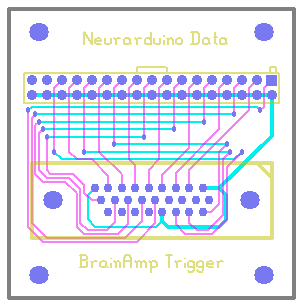
\includegraphics[width=0.5\textwidth]{layouts/adapter-brainamp-layout.png}
\end{center}
\caption{BrainAmp adapter PCB layout.}\label{fig-brainamp-pcb}
\end{figure}

%
% This is the end of the file.
